\section{Zielsetzung}
\label{sec:Zielsetzung}

Ziel des Versuches ist es das Anregungs- und Dämpfungsverhalten eines LRC-Schwingkreises
bei Wechselstrom verschiedener Frequenzen zu beschreiben.


\section{Theorie}
\label{sec:Theorie}

Zunächst wird der folgende Schwingkreis betrachtet, welcher durch einen
kurzen Strompuls in Gang gesetzt wird und danach abklingt.

\begin{figure}[H]
  \centering
  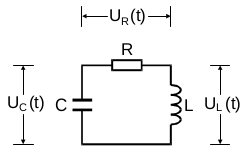
\includegraphics{content/images/V354.png}
  \caption{Gedämpfter L-R-C-Schwingkreis.}
  \label{fig:schwingkreis}
\end{figure}

Dieses Phänomen kann mathematisch durch die Überlagerung einer
einhüllenden und einer sinus/cosinus Funktion dargestellt werden.

\begin{figure}[H]
  \centering
  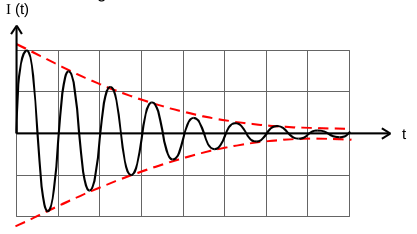
\includegraphics{content/images/dia.png}
  \caption{Dämpfungskurve des Stroms.}
  \label{fig:schwingkreis}
\end{figure}


\begin{align}
  \symbf{I} &= I_0 e^{-2\pi\mu t}
  \cdot\text{cos}\left(2\pi\nu t+\eta\right)\\
  \symbf{I}_\text{einhüllend} &= I_0 e^{-2\pi\mu t}
  \label{eqn:einhuellend}
\end{align}
